\section{Data and Preprocessing}
\subsection{Dataset}
The Fashion-MNIST is a dataset of Zalando article images, consisting of a training set of 60,000 samples and 10,000 test samples.
The dataset used here is a small portion of the original dataset, 10,000 training and 5,000 test samples.
Each sample is a 28x28 pixels gray-scale image with a label indicating the type of clothing item associated with each.
\newline

\begin{figure}[ht]
\centering
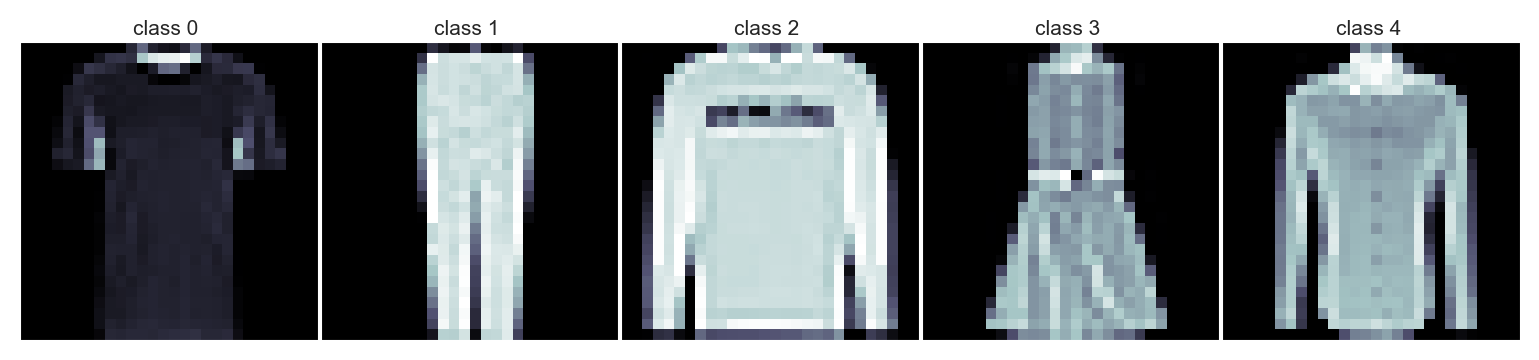
\includegraphics[scale=0.45]{figures_for_report/samples_from_classes}
\captionsetup{justification=centering,margin=2cm}
\caption{One sample from each class}
\end{figure}
\subsection{Naming Conventions}
The exploration of samples within each class gave rise to more appropriate names.
Class 0 became T-shirt etc.
Below is the naming conventions, which will be used throughout the report for better readability.  \\
\begin{table}[!ht]
  \footnotesize
  \centering
\begin{tabular}{ c c c c c c }
 \toprule
 \textbf{Label} & \textbf{0} & \textbf{1} & \textbf{2} & \textbf{3} & \textbf{4} \\
 \midrule 
 \textbf{Type of clothing} & T-shirt/Top & Trousers & Pullover & Dress & Shirt \\
 \bottomrule
\end{tabular} \\[0.2cm]
\captionsetup{justification=centering,margin=2cm}
\caption{Mapping from class-labels to clothing type}
\label{features}
\end{table}


\subsection{Data Cleaning}
The dataset provided was already in a cleaned state, which was verified by checking for missing values,
and checking that the pixel values were no greater than 255 and no smaller than 0.

\subsection{Preprocessing}
The pixels values were in the range $[0, 255]$.
This range was normalized to $[0, 1]$ by dividing each pixel by 255.
This was done to improve training time as working with small number is slightly faster computationally, and because neural networks prefers to work with small numbers.


% not sure if we need this tbh but it was recommended online see below
% https://sebastianraschka.com/Articles/2014_about_feature_scaling.html
% 1 of many sources for this ^ https://machinelearningmastery.com/how-to-manually-scale-image-pixel-data-for-deep-learning/ %
% https://tanthiamhuat.files.wordpress.com/2018/03/deeplearningwithpython.pdf pdf page 158 %

\subsection{Class Distribution}
Whether or not a machine learning model can learn to predict classes well depends to a high degree on how those classes are distributed within our training and training dataset.
Both the datasets are extremely balanced, with the test being fully balanced ($1000$ of each class).
This is illustrated on the plots below

\begin{figure}[ht]
\centering
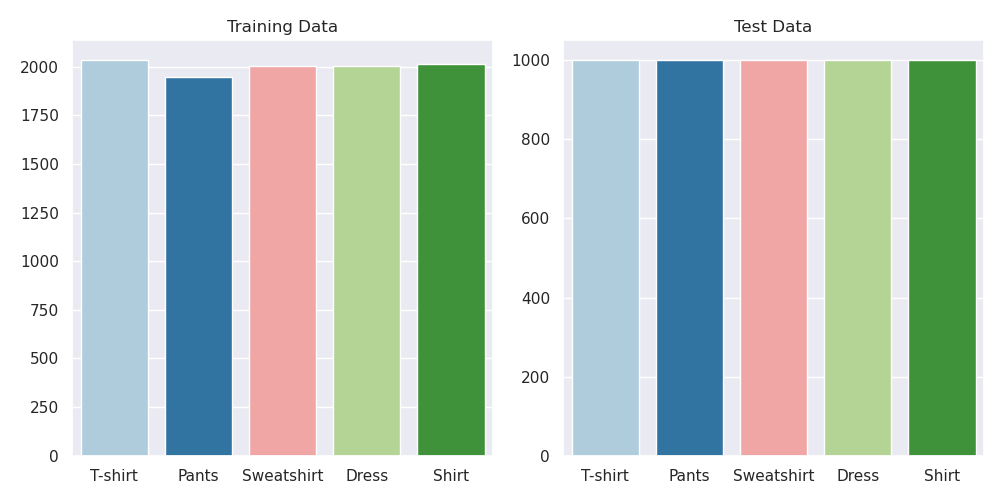
\includegraphics[scale=0.45]{figures_for_report/class_distribution}
\captionsetup{justification=centering,margin=2cm}
\caption{Distribution of clothing items in our training and test dataset}
\end{figure}

